\begin{appendices}

\chapter{Spectral Emissivity Library of Spoil Substrates}
\label{app:Library}

Spectral emissivity libraries contains valuable information about Earth surface materials, which can be utilised for validation and calibration purposes of airborne or satellite image data. Several libraries are currently available among which is also a spectral emissivity library of spoil substrates \cite{PP16}. This appendix introduces mentioned library in detail.

\section{Introduction}

Post-mining sites represent areas of large-scale and intensive disturbance. They can have significant impacts on the surrounding landscape in many countries of the world. Original ecosystems can be damaged or destroyed, and the restoration of ecosystem functions and services is necessary \cite{BH01}. Afforestation is widely used reclamation method. Many studies demonstrate that post-mining sites have a large potential for carbon sequestration if afforestation has been applied \cite{VF13, FL13, SL05, UL06}. This can contribute to mitigate the current increase in atmospheric $\mathrm{CO_2}$ concentrations.

During opencast mining a large amount of substrate above the coal layer is removed and relocated in heaps covering extensive areas. These heaps consist of material often excavated from depths of several hundred meters. This material is called spoil substrate and it can vary in its physical and chemical properties. The heterogeneity is largely affected by geology and the method of mining and heaping. For this reason the substrates differ substantially from recent soils. They often have extreme pH and may contain high concentrations of heavy metals, polyphenols (i.e., products of coal decomposition) and salt content. Such properties can significantly impact a success and/or speed of vegetation development at post mining sites. Therefore a proper knowledge on spoil substrate properties and distribution is necessary in land rehabilitation. 

Thermal infrared remote sensing can provide beneficial tools for monitoring of post-mining areas. Particularly, land surface emissivity (LSE) can be used for spoil substrates classification. In addition, physical and chemical properties can be estimated by spectral analysis of LSE. Land surface temperature (LST) is closely connected to soil moisture which is important for establishment of new ecosystems. All of this information is required when proper land reclamation should be applied. This can include mainly substrate mechanical treatment, such as trenching in order to regulate water regime, chemical treatment (e.g., liming), and selection of appropriate tree species.

LST is coupled with LSE and thus one quantity cannot be derived without knowledge of the second. These quantities cannot be explicitly derived from radiance measurement. The reason is that by observing radiance in N bands one gets N unknown emissivities plus one unknown temperature. Such a system of equations is underdetermined (i.e., more unknown than known variables). Several algorithms have been suggested to solve this problem \cite{LT13}. These algorithms either require knowledge of LSE in advance, or an estimate LSE as a part of their output. A library of spectral emissivities can be utilized for: 1) determination of LST, 2) material classification, and 3) LSE validation of airborne and satellite thermal remote sensing data.

This work describes a spectral library of spoil substrate emissivities from brown coal mining sites in the Czech Republic near towns of Sokolov, Chodov, Bílina and Ustí nad Labem (Figure \ref{fig:SpoilSubstratesMap}). The spectral library contains emissivities, soil pH in water and in KCl, soil conductivity, content of water soluble Na and K, Al and Fe in KCl, loss on ignition and content of polyphenols. In addition to all measured physical and chemical parameters, sample's latitude and longitude are listed. The dataset consists of 24 spoil substrate samples, which were homogenized by mixing and sieving before any sample analysis. The toxicity test and measurement of chemical properties are discussed at length in \cite{FK05}. Data collection for emissivity retrievals was performed outdoors in Petri dishes using a Fourier transform infrared (FTIR) spectrometer Model 102 (D\&P Instruments, United States). The emissivity of each sample was estimated by a spectral smoothing algorithm \cite{HJ98}.

\begin{figure*}[!t]
\centering
\includegraphics[width=0.95\linewidth]{pics/Chapter_05/map.pdf}
\vspace{1.5 em}
\caption{Locations of brown coal mining sites from which spoil substrate samples were extracted.}
\label{fig:SpoilSubstratesMap}
\end{figure*}

Datasets containing LSE are rare in comparison with datasets containing LST measurements. The most well-known spectral libraries containing emissivities are the ASTER Spectral Library \cite{BH09}, Johns Hopkins University Spectral Library \cite{SW91}, Arizona State University Spectral Library \cite{CB00}, United States Geological Survey Spectral Library \cite{CS16} and the Spectral Library of Urban Materials (SLUM) \cite{KS14}. However, these spectral libraries do not include neither geographical coordinates of samples nor representatives of spoil substrates. One example of a spectral library of emissivities from calibration/validation sites containing coordinates for each sample is described in \cite{SM09}. The dataset described in this paper is exceptional in its nature and location. 

The data presented in this paper were used in a study focused on mapping of spoil substrates for site re-cultivation \cite{Z14} as well as in a study discussing spoil substrates toxicity \cite{FK05}. The mining site was also mapped with the Airborne Hyperspectral Scanner (AHS) in visible, near infrared, shortwave infrared and longwave infrared regions for mineral classification purposes \cite{NK14}. Examples of emissivity spectra retrieved from AHS and their corresponding samples spectra extracted from the library are depicted in Figure \ref{fig:AHSvsFTIRcomparison}. Samples spectra from the library were spectrally resampled with respect to AHS response functions using weighted averages \cite{LT13}. Comparison of retrieved spectra in case of samples 11 and 19 shows good agreement in shape. Sample 12 exhibits deviations mainly between bands 3 and 4 (9.24 and \SI{9.68}{\micro\meter}). This can be explained by the fact that AHS pixel has 5x5 m pixel size and these pixels were not pure thus had more complex mineral composition than the collected samples. Discrepancies in magnitude can be addressed to imperfect atmospheric corrections or to different soil state during overflight.

\begin{figure}[!t]
	\centering
	\vspace{1em}
	\begin{subfigure}[t]{.3\linewidth}
		\centering
		\includegraphics[scale=1]{pics/Chapter_05/Sample_no_11.eps}
		\caption{}
	\end{subfigure}
	\hspace{1em}
	\begin{subfigure}[t]{.3\linewidth}
		\centering
		\includegraphics[scale=1]{pics/Chapter_05/Sample_no_12.eps}
		\caption{}
	\end{subfigure}
	\hspace{1em}
	\begin{subfigure}[t]{.3\linewidth}
		\centering
		\includegraphics[scale=1]{pics/Chapter_05/Sample_no_19.eps}
		\caption{}
	\end{subfigure}
	\vspace{1.5 em}
	\caption{Examples of corresponding emissivity spectra retrieved from AHS and from spectral library of spoil substrates’. Emissivity spectra from the library were measured by FTIR and they were resampled with respect to AHS response functions. }
	\label{fig:AHSvsFTIRcomparison}
\end{figure}

Any activity involving remote sensing over these mining sites can benefit from publicly releasing the spectral library of spoil substrates emissivity. Apart from remote sensing application, data in spectral library can be further analyzed for identifying relationships between a sample’s spectral emissivity and its chemical properties.

\section{Methods}

The study area is situated around two post mining districts: 1) Sokolov – coal-mining district near towns of Sokolov and Chodov (North-West Czech Republic) and 2) North Czech coal mining district near towns of Bílina and Ustí nad Labem (North Czech Republic). Open-pit mines produce large areas of tailings where spoil material was sampled. Claylike tertiary sediments dominate in these districts.

Spoil substrates were sampled from bare soil without vegetation. Samples contained negligible amounts of organic matter. Extracted samples were further homogenized by mixing and sieving trough a \SI{2}{\milli\meter} screen. Homogenized samples were divided into two groups, from which the first one was used for chemical analysis and the second one for toxicity testing. Samples set for chemical analysis were air dried and stored in a dark place at room temperature. Soil pH in water and in 1N KCl (which is \SI{74.56}{\gram} of potassium chloride diluted in \SI{1000}{\milli\liter} of water \cite{J03}) was measured using a pH meter with glass electrode in suspension. The suspension was prepared in 1:5 spoil to water ratio and 1:5 spoil to KCl ratio. Conductivity was measured in filtrated suspension using a conductometer. The suspension was prepared in 1:5 spoil to water ratio. Content of water soluble Na and K was also measured in filtrated water suspension (1:5 spoil to water ratio) using an ion selective electrode. Both suspensions were left to stay overnight. Al and Fe contents in 1N KCl eluate, (1:5 spoil to water ratio), were determined by spectrophotometer Spectra AA 640 (Varian, Australia). Loss on ignition was measured by burning spoil samples at \SI{600}{\celsius} for \SI{5}{\hour} h. This process is called ashing. To determine the amount of polyphenols, samples were kept in 80\,\% ethanol (1:5 spoil to ethanol ratio) and stayed for \SI{24}{\hour}. Samples were then filtrated and the polyphenol content was determined spectrophotometrically by Folin–Ciocalteau reagent at a wavelength of \SI{765}{\nano\meter} \cite{HL97}. Gallic acid was used as a standard for calibration. The polyphenol content was expressed as \SI{}{\milli\gram\per 100\gram} of soil. Toxicity was determined by enchytraeid toxicity test. The test is based on the population growth of pot worms in substrates. The details of the measurement are discussed in \cite{FK05}.

Spoil substrate emissivity measurements were collected with Designs and Prototypes Model 102 (United States) portable FTIR spectrometer. The measurements were performed outdoors under clear sky conditions during two consecutive days in the summer season. The spectroradiometer was pre-heated to maximum expected ambient day temperature during the nights before both measurement days. The samples were positioned on the south side of the spectrometer to avoid shadows. The fore-optic field-of-view was \SI{4.8}{\degree} and it was \SI{60}{\centi\meter} from the sample. Such a configuration resulted in a spot size of approximately 5 cm. Samples were put in a \SI{14}{\centi\meter} diameter Petri dish and were allowed to be heated up naturally in the sunlight. Sample temperatures ranged from \SI{40}{\celsius} to \SI{50}{\celsius}. Every sample was measured at three different spots. The measurement of one spot consisted of ten measurements, which were averaged. The resulting emissivity of each sample is the average of all three measurements. Sample temperature and emissivity were determined by a spectral smoothing algorithm, as described in \cite{HJ98}.

During the measurements the instrument was calibrated using two blackbodies at different temperatures. A cold blackbody was set to the ambient temperature (\SI{30}{\celsius}) and warm blackbody was set just above the sample temperature (40 -- \SI{50}{\celsius}). The calibration procedure during the first four spoil samples was done between the changing of each sample. The calibration procedure during the rest of the measurements was done between every fourth sample. Before every sample a measurement was made of a diffuse gold reflectance plate (Infragold from Labsphere Inc.), to compensate for downwelling radiance, as suggested in \cite{GV13}. The measurement of one sample along with instrument calibration and measurement of the diffuse gold reflectance plate took around 15 minutes. A description of the procedures for converting instrument response to radiance and compensating for downwelling radiance can be found in \cite{HJ98} and \cite{HK96}.

Some of the spoil substrate emissivity spectra are greater than one at certain wavelengths. This inaccuracy occurs at both ends of provided wavelengths interval (i.e. near \SI{8}{\micro\meter} and near \SI{14}{\micro\meter}). Data at these wavelengths are on the edge of atmospheric window and thus the cause of the inaccuracy is imperfect compensation for downwelling radiance. Samples with numbers 33, 34 and 38 are missing header information of latitude and longitude. Absent values are indicated by ‘NA’ string. In these cases the origin of the sample is specified with respect to closest town (either Bílina or Sokolov). We still find these data meaningful, since they can be used as spectral endmembers.


\section{Data Properties}

All of the samples contain varying amounts and types of clay minerals, as evidenced by their spectral emissivity features. Figure \ref{fig:SpectraPreview} depicts three examples of spoil samples taken from the spectral library. These spectra can be compared with spectra of similar materials extracted from Arizona State University Spectral Library \cite{CB00} and ASTER Spectral Library \cite{BH09}, which are illustrated in the Figure \ref{fig:SpectraPreview} as well. Sample 02 (Figure \ref{fig:SpectraPreview}a) is clay consisting mostly of kaolinite with significant dips at 8.90, 9.44, 9.90, and \SI{11.00}{\micro\meter}. Sample 06 (Figure \ref{fig:SpectraPreview}b) is coal combined with sand and clay. The emissivity spectrum of this sample contains kaolinite features mixed with a quartz feature at 8.47 and \SI{8.83}{\micro\meter}. The sample 33 (Figure \ref{fig:SpectraPreview}c) is bentonite rich for montmorillonite. Montmorillonite has typical dip in spectral emissivity at \SI{9.43}{\micro\meter}. The spectral emissivity library of spoil substrates includes also image providing a preview of all samples in library similar to images shown in Figure \ref{fig:SpectraPreview}.

\begin{figure}[!t]
	\centering
	\vspace{1em}
	\begin{subfigure}[t]{.3\linewidth}
		\centering
		\includegraphics[scale=1]{pics/Chapter_05/Sample_no_02.eps}
		\caption{}
	\end{subfigure}
	\hspace{1em}
	\begin{subfigure}[t]{.3\linewidth}
		\centering
		\includegraphics[scale=1]{pics/Chapter_05/Sample_no_06.eps}
		\caption{}
	\end{subfigure}
	\hspace{1em}
	\begin{subfigure}[t]{.3\linewidth}
		\centering
		\includegraphics[scale=1]{pics/Chapter_05/Sample_no_33.eps}
		\caption{}
	\end{subfigure}
	\vspace{1.5 em}
	\caption{Spectra of three samples taken from the spectral emissivity library of spoil substrates: (a) sample 02 representing clay rich for kaolinite; (b) sample 06 representing coal combined with sand and clay; (c) sample 33 representing bentonite. Kaolinite and montmorillonite spectra were extracted from Arizona State University Spectral Libary \cite{CB00} and quartz spectra was extracted from ASTER Spectral Library \cite{BH09}. Kaolinite spectrum is scaled for clarity reasons.}
	\label{fig:SpectraPreview}
\end{figure}

Thermal infrared remote sensing can be used for classification of spoil substrates and for determination of their physical and chemical properties. The spectral library presented in this paper can ease and enhance all these activities. Obtaining this information together with LST is valuable for selection and monitoring of restoration process at post-mining sites. 

\section{Data Description}

The spectral library consists of 24 ASCII files. Each file describes one spoil substrate. Individual files are named according to the sample number. Files consist of a file header and spectral emissivities. Both file parts are described in the subsections below.

\subsection{Header}

The format of the header is similar to the format of the ASTER Spectral Library header \cite{BH09}. Each file contains 26 lines of header, which includes available sample information. The header is divided into four sections separated by empty lines. First part contains 9 lines discussing sample classification, particle size and sample origin. Sample origin is expressed by latitude and longitude on the reference ellipsoid WGS84. This information is summarized in the following fields:

\begin{enumerate}
	\item	Name
	\item Type
	\item Class
	\item Particle size
	\item Sample No
	\item Owner
	\item Origin
	\item Latitude
	\item Longitude
\end{enumerate}

A second section contains information about sample toxicity and chemical properties. The unit of each quantity is indicated in square brackets after quantity name. This header section contains following fields:

\begin{enumerate}
	\item toxicity
	\item pH in H20
	\item pH in KCl
	\item conductivity
	\item water soluble Na
	\item water soluble K
	\item Al in KCl
	\item Fe in KCl
	\item loss on ignition
	\item polyphenol content
\end{enumerate}

A third section contains reference to \cite{FK05}, which discusses toxicity measurement and chemical analysis. Finally, the fourth header section contains the names of two columns, in which the following spectral emissivity data are aligned. Metadata in each header line contains an attribute name followed by a colon (ASCII Character 3A) and tab (ASCII Character 09) and then the corresponding value.

\subsection{Spectral Emissivity}

After the header part, the file continues on lines 27 – 213 with spectral emissivity data aligned in two columns. As header file indicates, the first column contains wavelength in micrometers and the second column contains corresponding emissivity value. Values in each row are separated by tab. The emissivity of each sample is provided in wavelengths interval from \SI{8}{\micro\meter} to \SI{14}{\micro\meter}. Sampling in this interval is non-linear. Spectral emissivities contained in the spectral library are depicted in Figures \ref{fig:SpoilSubstratesPreviewPt1} and \ref{fig:SpoilSubstratesPreviewPt2}. Spectral emissivity library is part of the supplementary materials to the manuscript \cite{PP16}.

\begin{figure*}[!t]
\centering
\includegraphics[width=0.95\linewidth]{pics/Chapter_05/spectral_library_pt1.eps}
\vspace{1.5 em}
\caption{Depiction of samples' emissivity spectra included in the library of spoil substrates.}
\label{fig:SpoilSubstratesPreviewPt1}
\end{figure*}

\begin{figure*}[!t]
\centering
\includegraphics[width=0.95\linewidth]{pics/Chapter_05/spectral_library_pt2.eps}
\vspace{1.5 em}
\caption{Depiction of samples' emissivity spectra included in the library of spoil substrates.}
\label{fig:SpoilSubstratesPreviewPt2}
\end{figure*}